\chapter{Feature descriptor} \label{sec:feature_descriptor}

For a computer, a picture is represented as a 2-D or 3-D array.

The color is one of the key components of a food item, thus it is widely applied for classification. Color statistics are commonly used, such as the first and second moment values for different channels. It can be computed for multiple color representations (RGB, HSV, gray, YCrCb or L*a*b* space).

Another import feature of the food is the tetxure. Numerous texture feature can be used such as Gabor filters. As already presented, the local binary pattern is also applied.

\section{Local binary pattern}

% http://www.pyimagesearch.com/2015/12/07/local-binary-patterns-with-python-opencv/

Local binary pattern is a visual descriptor for texture composition of an image, first presented in 2002 in \cite{Ojala2002} (although the concept of LBPs were introduced as early as 1993).

\subsection{Gray-scale LBP}

The figure \ref{fig:lbp_process} represents an example of the LBP in which the LBP code of the center pixel (in red color and value 20) is used as a local intensity threshold : the neighbour pixels whose intensities are equal or higher than the center pixel’s are labeled as ”1”; otherwise as ”0”. Then, starting always from the same point, we can transform this binary string to decimal and is used to describe the central pixel. In this example we start at the top-right point and work our way clockwise accumulating the binary string as we go along and obtain the value 24.

\begin{figure}[h]
    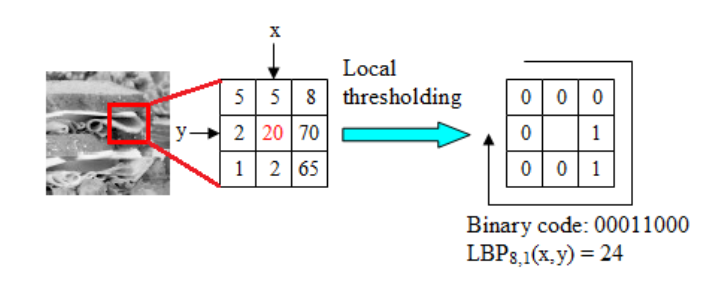
\includegraphics[scale=0.55]{img/lbp}
    \caption{Illustration of the LBP descriptor's process}
    \label{fig:lbp_process}
\end{figure}

We adopt the following notation. Given a pixel $c = (x_c, y_c)$, the value of the $LBP$ code of $c$ is defined as:
$$LBP_{P, R} (x_c, y_c) = \sum_{p = 0}^{P - 1} s (g_p - g_c) 2^p$$
where:
\begin{itemize}
    \item $p$ is a neighbour pixel of $c$ and the distance from $p$ to $c$ does not exceed $R$. Thus, $R$ is the radius of a circle centered in $c$ and $P$ is the numbered of sampled points.
    \item $g_p$ and $g_c$ are the gray values (intensities) of $p$ and $c$
    \item $s(x)$ is the function defined as:
    \begin{equation}
    s(x) =
    \begin{cases}
    1 & \text{if $x \geq 0$}\\
    0 & \text{otherwise} \\
    \end{cases}
    \end{equation}
\end{itemize}

In Fig. \ref{fig:lbp_process}, $R$ and $P$ are 1 and 8 respectively.

The number of histograms bins for $LBP_{P, R}$ is $2^P$.

\subsection{Uniform LBP}

This algorithm has been enhanced to make it rotation invariant. Still in \cite{Ojala2002}, the authors introduce the notion of uniform LBP. A LBP is considered to be uniform if it has at most two bitwise transitions (0 to 1 or 1 to 0 transitions in the binary word). 

For example, the pattern \textit{01000000}  (2 transitions) and \textit{11111110} (1 transition) are both considered to be uniform. For a $LBP_{P, R}$, there is $p + 1$ possible uniforms.

Non-uniform LBP are considered as noise and are assigned the same constant value.

Thus, for uniform LBP, we use the formula:

$$
LBP_{P, R}^{uni} (x_c, y_c) = 
\begin{cases} \displaystyle
\sum_{p = 0}^{P - 1} s (g_p - g_c) 2^p & \text{if uniform} \\
P + 1 & \text{otherwise} \\
\end{cases}
$$

\section{Color descriptor}
\subsection{Color histogram}

HSV space is composed of:
\begin{itemize}
    \item \textbf{Hue} channel: represents the dominant spectral component—color in its pure form, as in green, red, or yellow
    \item \textbf{Saturation} channel: represents the white added to the pure color (the Hue)
    \item \textbf{Value} channel: represents the brightness of the color
\end{itemize}

Hue and Saturation corresponds to the chromaticity of the colour. For the joint histogram (2D histogram), the H and S channels are used as value is dependant of the condition where the picture were taken, thus is not interesting.

The coordinate system is cylindrical, and is often represented by a subspace defined by a six-sided inverted pyramid. The top of the pyramid corresponds to, with the “white” at the center. The hue is measured by the angle around the vertical axis, with red corresponding to 0. The saturation
ranges from 0 at the center to 1 on the surface of the pyramid. An inverted cone is also used to denote the subspace instead of the pyramid.

\subsection{Color moments}

\subsection{The first two moments}

For a discrete random variable $X$, the first two moments are defined as:
\begin{itemize}
    \item \textbf{Expected value}: $$\E \left[ X \right] = \mu = \sum_{i = 1}^{n} p_i x_i $$
    \item \textbf{Variance}:  $$ \Var (X)= \E \left[ (X - \E \left[ X \right] )^2 \right] =\sum _{i=1}^{n} p_i (x_{i} - \mu )^{2} $$
\end{itemize}

\subsection{Hu moments}

\subsubsection{Raw moments}

For a two-dimensional continuous function f(x,y) the moment (sometimes called \enquote{raw moment}) of (p + q)th order is defined as: 
$$ M_{pq}=\int \limits _{-\infty }^{\infty }\int \limits _{-\infty }^{\infty }x^{p}y^{q}f(x,y) dx dy $$
for $p$ and $q \in \N $.

\subsubsection{Central moments}

And the central moments are :
$$\mu_{pq}=\int \limits_{-\infty }^{\infty }\int \limits _{-\infty}^{\infty} (x- \bar{x})^{p}(y - \bar{y})^{q} f(x,y) dx dy $$
with $\bar{x}=\frac{M_{10}}{M_{00}}$ and $\bar{y}=\frac{M_{01}}{M_{00}}$

\subsubsection{Normalized central moments}

The normalized central moments are:
$$ \eta_{ij}=\frac{\mu _{ij}}{\mu_{00}^{\gamma}} $$
where $\gamma = 1 + \frac{I + j}{2}$ for $i + j \geq 2$.

\subsubsection{Definition of the Hu moments}

On the base of those Moments, Hu in \cite{Hu1962} introduced 7 Moments which are invariant for translation, rotation and resizing:
\begin{align*}
    I_{1} = & \eta _{20}+\eta _{02} \\
    I_{2} = & (\eta _{20}-\eta _{02})^{2}+4\eta _{11}^{2} \\
    I_{3} = & (\eta _{30}-3\eta _{12})^{2}+(3\eta _{21}-\eta _{03})^{2} \\
    I_{4} = & (\eta _{30}+\eta _{12})^{2}+(\eta _{21}+\eta _{03})^{2} \\
    \begin{split}
        I_{5} = & (\eta _{30}-3\eta _{12})(\eta _{30}+\eta _{12})[(\eta _{30}+\eta _{12})^{2}-3(\eta _{21}+\eta _{03})^{2}] \\
        & +(3\eta _{21}-\eta _{03})(\eta _{21}+\eta _{03})[3(\eta _{30}+\eta _{12})^{2} -(\eta _{21}+\eta _{03})^{2}]
    \end{split} \\
    I_{6} = & (\eta _{20}-\eta _{02})[(\eta _{30}+\eta _{12})^{2}-(\eta _{21}+\eta _{03})^{2}]+4\eta _{11}(\eta _{30}+\eta _{12})(\eta _{21}+\eta _{03}) \\
    \begin{split}
        I_{7} = & (3\eta _{21}-\eta _{03})(\eta _{30}+\eta _{12})[(\eta _{30}+\eta _{12})^{2}-3(\eta _{21}+\eta _{03})^{2}] \\
        & - (\eta _{30}-3\eta _{12})(\eta _{21}+\eta _{03})[3(\eta _{30}+\eta _{12})^{2}-(\eta _{21}+\eta _{03})^{2}]
    \end{split} \\
\end{align*}

\section{Bag-of-Words}
\subsection{Process}

\textbf{Bag-of-Words} \textit{BoW}, also called Bag of features, is a feature descriptor method inspired by information retrieval from textual documents.

As illustrated in Fig. \ref{fig:bow_process}, the main steps are:
\begin{itemize}
    \item On each picture, keypoints are detected. In my case, I use a dense grid of evenly spaced points at a fixed scale and orientation.
    \item For every keypoint, a feature vector  is generated. we describe it, SIFT (scale invariant feature transform).
    \item We generate the fix number of visual words that compose our codebook.
    \item We express each image as an histogram of these words' appearance.
\end{itemize}

The combination of a dense grid and SIFT is commonly called dense SIFT. It has been showed to have greater accuracy than using SIFT for keypoint detection and description.

\begin{figure}
    \centering
    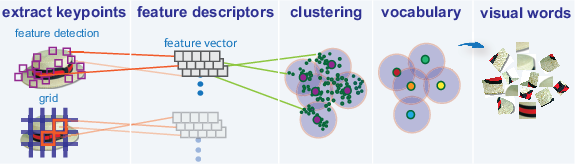
\includegraphics[scale=0.9]{img/bow.png}
    \caption{Illustration of the Bag-Of-Visual-Words model}
    \label{fig:bow_process}
\end{figure}

\subsection{SIFT descriptor}

A SIFT descriptor of a local region (keypoint) is a 3-D spatial histogram of the image gradients as presented in the figure \ref{fig:sift_descriptor}. The gradient at each pixel is regarded as a sample of a three-dimensional elementary feature vector, formed by the pixel location and the gradient orientation. Samples are weighed by the gradient norm and accumulated in a 3-D histogram h, which (up to normalization and clamping) forms the SIFT descriptor of the region. An additional Gaussian weighting function is applied to give less importance to gradients farther away from the keypoint center.

\begin{figure}
    \centering
    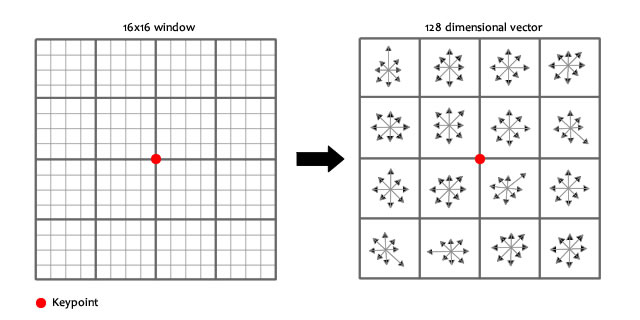
\includegraphics[scale=0.5]{img/sift_descriptor.jpg}
    \caption{Illustration of SIFT as a local image descriptor}
    \label{fig:sift_descriptor}
\end{figure}

\subsection{K-mean clustering}

Given a set of observations $(x_1, x_2, …, x_n)$, where each observation is a d-dimensional real vector, k-means clustering aims to partition the $n$ observations into $k$ $(k \leq n)$ sets $S = {S_1, S_2, …, S_k}$ so as to minimize the within-cluster sum of squares (sum of distance functions of each point in the cluster to the K center). In other words, its objective is to find:

\begin{equation} \label{eq:kmean_objective}
    \underset {S}{\argmin} \sum _{i=1}^{k} \sum _{x \in S_{i}} \left\| x - \mu_{i} \right\|^{2}
\end{equation}

Problem, the exact solution is a NP hard problem. That's why, we can use Lloyd's heuristic algorithm to compute an estimation.

It is an iterative method that find a local minima of the Eq. \ref{eq:kmean_objective}:

\begin{enumerate}
    \item A set of $k$ initial \enquote{means} is choosen randomly within the data domain $M = \{m_1, m_2, \ldots, m_k \}$
    
    \item Then, k clusters are created by associating every observation with the nearest mean.
    $$ \forall i \in \{ 1, \ldots, k \}, ~~ S_{i}^{(t)}= \big \{ x_{p}:{\big \|}x_{p}-m_{i}^{(t)}{\big \|}^{2}\leq {\big \|}x_{p}-m_{j}^{(t)}{\big \|}^{2} ~ \forall j \in \{ 1, \ldots, k \} \big \}$$
    
    \item The centroid of each of the k clusters becomes the new mean.
    $$ \forall i \in \{ 1, \ldots, k \}, ~~ m_{i}^{(t+1)}=\frac {1}{\lvert S_{i}^{(t)} \rvert } \sum _{x_{j} \in S_{i}^{(t)}} x_{j} $$
    
    \item Repeats step 2 and 3 until $M$ not longer changes.
\end{enumerate}

The centroid results and number of iterations are highly dependant of the initial centroid.

As a result, the computation is often done several times, with different initializations of the centroids. One method to help address this issue is the k-means++ initialization scheme, which has been described in \cite{Arthur2007}. This initializes the centroids to be (generally) distant from each other, leading to provably better results than random initialization.
